\chapter{MATERIALS AND METHODS}

\section{Consensus \emph{S. cerevisiae} Metabolic Model}
Variety of \emph{S. cerevisiae} genome-scale metabolic models have been used since 2003, and each reconstructed model introduced more manual curations, increasing gene numbers from annotations and better predictions regarding the previous ones \cite{lopes2017genome}. A consensus genome-scale metabolic model of \emph{S. cerevisiae}, Yeast8, is presented in an open-source, version-controlled maintainable way in 2019, claiming that the model can be represented and investigated in a systematic way using Git (https://git-scm.com/) and GitHub (https://github.com/) as a hosting service for the model repository \cite{lu2019consensus}. Systematic way of Yeast8 enables to study simultaneously in collaborative studies, provides record keeping of model changes, version updates, where each version of it can be released periodically and accessible all the time (Figure \ref{fig:yeast8_github}).

Yeast8 model can be considered as an updated version of Yeast7 \cite{aung2013revising} with additional correactions based on the annotations available in KEGG and ChEBI, and several gene inclusions from the model iSce926 \cite{chowdhury2015using}. Final version of Yeast8 to date, version 8.3.4 released on July 28, has 3991 reactions, 2691 metabolites, 1149 genes and 14 intracellular compartments. Additional statistical analysis on its stoichiometric matrix can be seen in Figure \ref{fig:modelstats}.

All simulations in the Methods section are done on the model Yeast8 v8.3.4 which is hosted in Github (https://github.com/SysBioChalmers/yeast-GEM). Optimization problems were solved with the COBRA Toolbox v3.0.6 and the RAVEN Toolbox v2.3.1 in MATLAB (version 9.7.0.1216025 (R2019b)), using Gurobi solver (version 8.1.1).

\begin{figure}[H]
\begin{center}
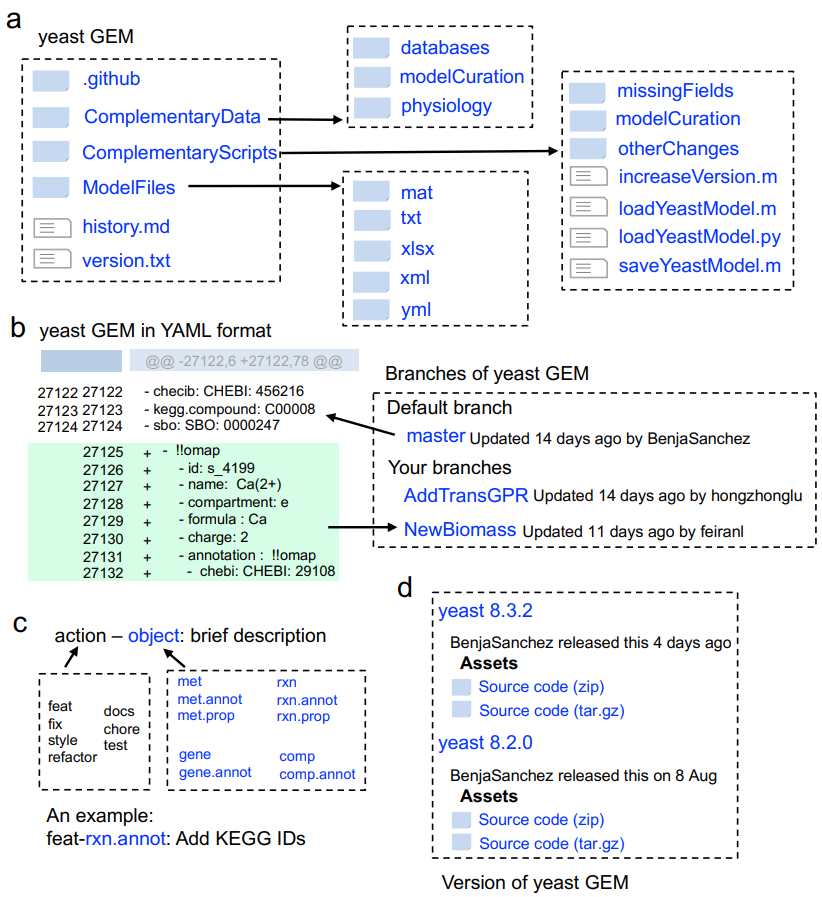
\includegraphics[width=1\columnwidth]{yeast8_github.png}
\end{center}
\caption[Repository of yeast GEM on GitHub]{Repository of yeast GEM on GitHub \cite{lu2019consensus}.}
\label{fig:yeast8_github}
\end{figure}

\begin{figure}[H]
\begin{center}
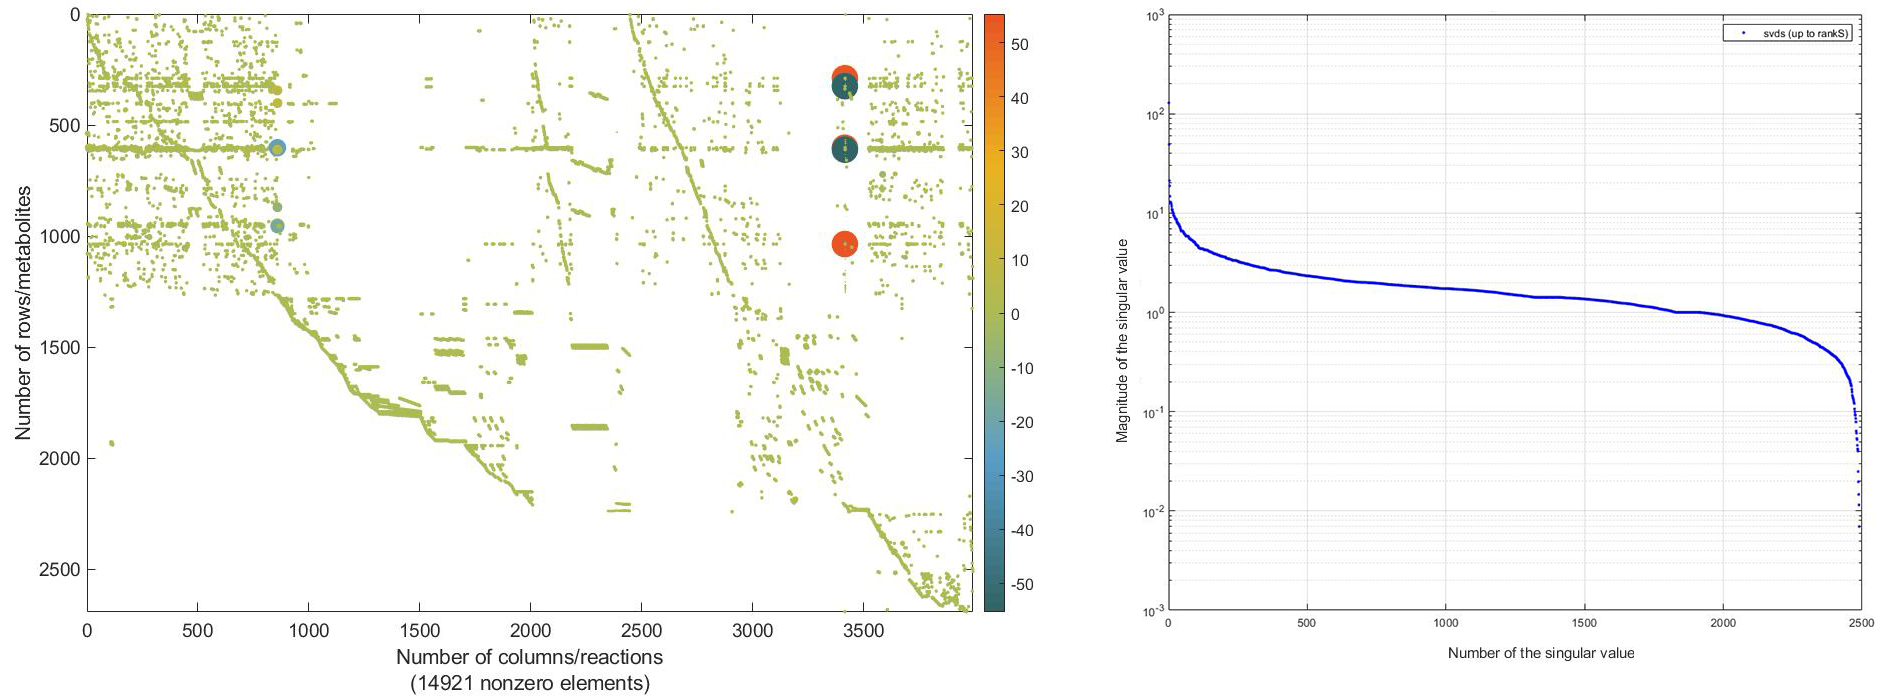
\includegraphics[width=1\columnwidth]{modelstats.png}
\end{center}
\caption[Coefficients and singular values of the stoichiometric matrix of Yeast8]{Coefficients and singular values of the stoichiometric matrix of Yeast8}
\label{fig:modelstats}
\end{figure}



\section{Experimental Data Acquisition} \label{experimentaldataacquisition}
Extracellular metabolomics data are obtained from Cakar's Lab \cite{arslan2018physiological}. Briefly, they perform ethyl methane sulfonate (EMS) mutagenesis  on the prototrophic \emph{Saccharomyces cerevisiae} strain CEN.PK 113-7D (MATa, MAL2-8c, SUC2) to increase the genetic diversity as a selection strategy by evolutionary engineering. Cells were inoculated in 2\% Yeast Minimal Media (YMM), and the extracellular concentrations of glucose, ethanol, glycerol and acetate were measured at different time points. OD\textsubscript{600} values were determined by a spectrophotometer. Additionally, cell dry weight analysis was conducted to determine biomass production.

Measured OD\textsubscript{600} values and dry weights of the reference strains (without mutagenesis, referred as wild-type in the models) of all ALE experiments were used in this study, and are collected in  Table \ref{table:experimental_OD600s_and_growths}. Experimental extracellular metabolite concentrations are also collected in Table \ref{table:experimental_data}, and compared with the computational simulation results in the discussions.

\begin{table}[H]
\caption[Measurements of extracellular concentrations \cite{surmeli2019evolutionary}]{Measurements of extracellular concentrations \cite{surmeli2019evolutionary}.}
\begin{center}
\begin{tabular}{|c|c|c|c|c|}
   \hline
  \textbf{Time(h)} & \textbf{Glucose(g/L)} & \textbf{Ethanol(g/L)} & \textbf{Glycerol(g/L)} & \textbf{Acetate(g/L)} \\
    \hline
  0                 & 19.99            & 0                & 0                 & 1.08             \\
  3                 & 17.98            & 0.58             & 0.02              & 1.24             \\
  6                 & 15.85            & 1.2              & 0.06              & 1.16             \\
  9                 & 12.21            & 3.39             & 0.18              & 1.37             \\
  12                & 9.18             & 7.97             & 0.61              & 2.45             \\
  15                & 0.4              & 8.17             & 0.69              & 2.46             \\
  27                & 0                & 8.28             & 0.76              & 2.6              \\
  46                & 0                & 8                & 0.77              & 2.45             \\
  50                & 0                & 6.62             & 0.64              & 2.02             \\
  54                & 0                & 5.74             & 0.55              & 1.73             \\
  58                & 0                & 5.46             & 0.54              & 1.74             \\
  72                & 0                & 3.72             & 0.49              & 1.33            \\
   \hline
\end{tabular}
\label{table:experimental_data}
\end{center}
\end{table}

\begin{table}[H]
\caption[Measured OD\textsubscript{600} and cell dry weight values of reference strain \cite{surmeli2019evolutionary}]{Measured OD\textsubscript{600} and cell dry weight values of reference strain \cite{surmeli2019evolutionary}.}
\begin{center}
  \begin{tabular}{|c|c|c|c|}
 \hline
  \textbf{Time (h)} & \textbf{OD600} & \textbf{ln(OD600)} & \textbf{Cell DW (g/L)} \\
  \hline
  0                 & 0.21           & -1.560647748       & -                      \\
  3                 & 0.53           & -0.634878272       & -                      \\
  6                 & 1.76           & 0.565313809        & 0.9                    \\
  7.5               & 2.66           & 0.978326123        & -                      \\
  9                 & 4.46           & 1.495148766        & 1.9                    \\
  12                & 5.31           & 1.669591835        & -                      \\
  15                & 5.88           & 1.771556762        & -                      \\
  18                & 5.83           & 1.763017           & 2.32                   \\
  21                & 6.07           & 1.803358605        & -                      \\
  24                & 5.87           & 1.769854634        & -                      \\
  30                & 6.14           & 1.814824742        & 2.26                   \\
  40                & 6.44           & 1.86252854         & -                      \\
  46                & 6.36           & 1.850028377        & -                      \\
  50                & 6.3            & 1.840549633        & -                      \\
  54                & 6.55           & 1.87946505         & -                      \\
  63                & 6.54           & 1.877937165        & -                      \\
  67                & 6.88           & 1.928618652        & -                      \\
  72                & 6.97           & 1.941615225        & 2.66                  \\
   \hline
  \end{tabular}
\label{table:experimental_OD600s_and_growths}
\end{center}
\end{table}


As the slope in the curve of lnOD\textsubscript{600} as a function of time gives the growth rates of cells, natural logarithm of OD\textsubscript{600} values were calculated to obtain specific growth rates by using the equation \ref{eq:growthrates}.
  \begin{equation}
      \ \mu = \frac{\Delta \ln{OD_{600}}}{\Delta t}
      \label{eq:growthrates}
  \end{equation}

In order to determine uptake and secretion rates of the metabolites, the steady-state assumption is applied in three hours intervals as the shortest measured time-points. Missing data on cell dry weights are estimated from the OD\textsubscript{600} values, and these cell dry weight data is used to calculate fluxes (in the unit of mmol/gDWh). Measurement of the cell dry weight at the 3rd hour was crucial for the steady-state assumption, however data was not available from the experiments. Curve trend of the OD\textsubscript{600} plot is used as a guide to estimate cell dry weight (Figure \ref{fig:GrowthGraphs}).
\begin{figure}[H]
  \begin{center}
  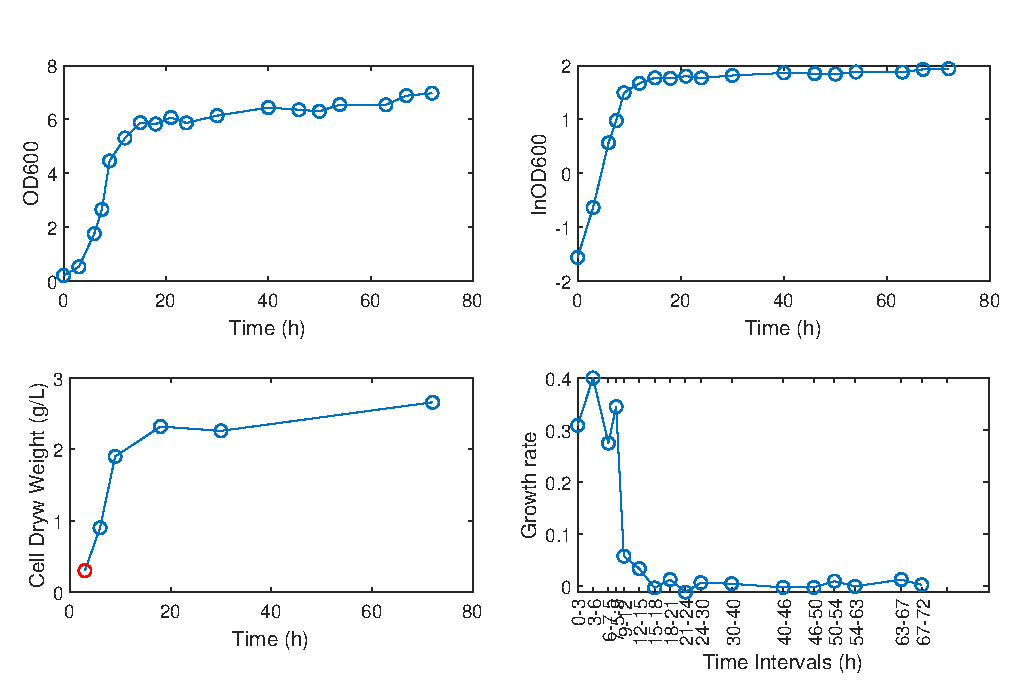
\includegraphics[width=1\columnwidth]{GrowthGraphsSmall.eps}
  \end{center}
  \caption[OD\textsubscript{600}, lnOD\textsubscript{600}, cell dry weights and growth rates]{OD\textsubscript{600}, lnOD\textsubscript{600}, cell dry weights and growth rates graphs. Estimated missing cell dry weight data is shown in red color.}
\label{fig:GrowthGraphs}
\end{figure}



\section{Flux Balance Analysis}
Flux balance analysis (FBA) assumes that the living cells act as they optimized their lives towards some goal, and as if they were at steady state. To be more clear, steady-state assumption indicates that the metabolites are both produced and consumed at the same rate in a cell, without an accumulation. Therefore, in this system, metabolites are constrained by only the stoichiometric coefficients arise from mass balance of metabolites. FBA solves a set of ordinary differential equations regarding to the stoichiometric matrix:
\begin{equation}
 \ S_{m \times n} \cdot v=0
\end{equation}
\noindent where S is the matrix of the stoichiometric reaction coefficients with m number of metabolites (as rows) and n number of reactions (as columns), and v is the vector of all associated reaction fluxes (mmol/gDWh). Because the matrix S usually has more reactions than metabolites (m<n), the system can result multiple solutions, and being called an underdetermined system (read more on Section \ref{metabolicnetworks}). To solve it for an optimal solution, additional constraints or an objective function is required.

A "growth reaction" is usually included in the reactions of the system to represent the "goal" in the definition of living systems. Growth reactions act as the final consumption of metabolites necessary for the biomass production or cell replication. Additional to the growth, several exchange reactions (uptake or secretion of metabolites from or into extracellular space) are also included. Since the concentrations of extracellular metabolites are measurable experimentally, constraints can be applied to exchange reaction fluxes to shrink solution space. The more constraints introduced into the system, such as reversibility of reactions or known rate values, the more smaller solution space results. The growth reaction is usually used as an objective function to determine a unique solution from this solution space. The linear problem appears as:
\begin{align}
 \ \text{max}_v \quad & c^T \cdot v \\
 \label{eq:fba}
 \ \text{subject to} \quad & S_{m \times n} \cdot v=0 \\
 \ & v_{lb} \leq v \leq v_{ub}
\end{align}
\noindent where c is the objective function vector, v is the vector of fluxes, S is the stoichiometric matrix as in above equation. Subscripts lb and ub are the lower and upper boundaries on v. These constraints define a feasible region of the problem. The coefficients of the biomass constituents are defined as the same as the batch conditions in the reference article \cite{nilsson2016metabolic}, for the reason that detailed knowledge is not available in the acquired experimental data (see section \ref{experimentaldataacquisition}). The coefficients for the final biomass equation can be found in the Table \ref{table:biomass_coefficients}.

\begin{table}[H]
\small
\caption[Biomass coefficients]{Biomass formulation that are used in the Yeast8}
\begin{center}
  \begin{tabular}{|p{3cm}|p{11.5cm}|}
  \hline
  \textbf{Products} & \textbf{Components} \\ \hline
  Biomass      & lipid + protein + carbohydrate + RNA + DNA + cofactor + ion \\ \hline
    Lipid   & lipid backbone + lipid chain \\ \hline
  Lipid Backbone  & 0.0063196 1-phosphatidyl-1D-myo-inositol backbone +
  0.024311 ergosterol + 0.0062241 ergosterol ester backbone  +
  0.0013536 fatty acid backbone +
  0.0054422 phosphatidyl-L-serine backbone +
  0.023579 phosphatidylcholine backbone  +
  0.006337 phosphatidylethanolamine backbone +
  0.006271 triglyceride backbone \\ \hline
  Lipid Chain  & 0.0073947 C16:0 chain +
  0.021702 C16:1 chain +
  0.0020726 C18:0 chain +
  0.0079624 C18:1 chain \\ \hline
  Protein      & 0.57284 Ala-tRNA(Ala) +
  0.20064 Arg-tRNA(Arg) +
  0.12698 Asn-tRNA(Asn) +
  0.37145 Asp-tRNA(Asp) +
  0.0082405 Cys-tRNA(Cys) +
  0.1316 Gln-tRNA(Gln) +
  0.37682 Glu-tRNA(Glu) +
  0.36258 Gly-tRNA(Gly) +
  0.08278 His-tRNA(His) +
  0.2406 Ile-tRNA(Ile) +
  0.37007 Leu-tRNA(Leu) +
  0.35734 Lys-tRNA(Lys) +
  0.063302 Met-tRNA(Met) +
  0.16718 Phe-tRNA(Phe) +
  0.20564 Pro-tRNA(Pro) +
  0.23148 Ser-tRNA(Ser) +
  0.23897 Thr-tRNA(Thr) +
  0.035459 Trp-tRNA(Trp) +
  0.12735 Tyr-tRNA(Tyr) +
  0.33037 Val-tRNA(Val) \\ \hline
  Carbohydrate   & 0.68454 (1->3)-beta-D-glucan +
  0.22871 (1->6)-beta-D-glucan +
  0.33052 glycogen +
  0.65017 mannan +
  0.12646 trehalose \\ \hline
  RNA   & 0.044535 AMP +
  0.043276 CMP +
  0.044535 GMP +
  0.057992 UMP \\ \hline
  DNA   & 0.0036 dAMP +
  0.0024 dCMP +
  0.0024 dGMP +
  0.0036 dTMP \\ \hline
  Cofactors   & 0.00019 coenzyme A +
  1e-05 FAD +
  0.00265 NAD +
  0.00015 NADH +
  0.00057 NADP(+) +
  0.0027 NADPH +
  0.00099 riboflavin +
  1.2e-06 TDP +
  6.34e-05 THF +
  1e-06 heme a \\ \hline
  Ions   & 3.04e-05 iron(2+) +
  0.00363 potassium +
  0.00397 sodium +
  0.02 sulphate +
  0.00129 chloride +
  0.00273 Mn(2+)  +
  0.000748 Zn(2+) +
  0.000217 Ca(2+) +
  0.0012425 Mg(2+) +
  0.000659 Cu2(+) \\ \hline

  \end{tabular}
\label{table:biomass_coefficients}
\end{center}
\end{table}


There are multiple available command-line functions to solve a linear programming problem such as \emph{linprog()} function of MATLAB, \emph{optimizeCbModel()} function of the COBRA Toolbox, or \emph{solveLP()} function of the RAVEN Toolbox with using variety of solvers such as GLPK, GUROBI or IBM cplex.

In order to simulate batch conditions where the minimal yeast medium is used, all the exchange reactions in the model are first blocked (lower bounds are set to 0). Then, only the exchange reactions of the ions that are available to the cells in the experimental design (ammonium, phosphate, sulphate, iron(2+), H+, water, chloride, Mn\textsuperscript{2+}, Zn\textsuperscript{2+}, Mg\textsuperscript{2+}, sodium, Cu2\textsuperscript{2+}, Ca\textsuperscript{2+}, potassium) are set free (lower bounds are set to -1000), meaning that cells can uptake then as needed.


\section{Integration of Enzymatic Constraints}

Solution space of the yeast model can be further constrained by limiting fluxes of reactions with integration of enzymatic information by using GECKO (GEM with Enzymatic Constraints using Kinetic and Omics data) method \cite{sanchez2017improving}.  In GECKO methodology, if a reaction has an annotated enzyme, enzyme entity itself is included in the same reaction equation. Stoichiometric coefficient of this entity is defined by its kinetic information and abundance in the cell (Figure \ref{fig:gecko1}). S matrix of the system is expanded with the addition of new rows for the enzymes and new columns for the each enzyme's usage.

\begin{figure}[H]
\begin{center}
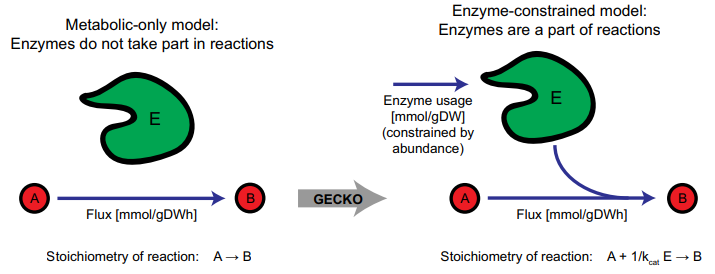
\includegraphics[width=1\columnwidth]{gecko1.png}
\begin{align}
\label{eq:geckoreaction}
 \ A \xrightarrow{E_i} B \\
 \label{eq:gecko}
 \ A + n_{ij}E_i \xrightarrow{} B
\end{align}
\end{center}
\caption[GECKO methodology to integrate enzymatic constraints]{GECKO methodology to integrate enzymatic constraints.}
\label{fig:gecko1}
\end{figure}

The idea behind this methodology arises from the biochemical constraints, such that the maximum rate of a reaction is smaller or equal to its enzyme's turnover number and the concentration (mmol/gDW).
\begin{align}
 \label{eq:gecko_simple}
 \ v_{j} \leq k_{cat}^{ij} \cdot [E_{i}]
\end{align}
Enzymes in the reaction equations must be considered as pseudo-metabolites because they do not affect the mass balance of the reaction, i.e., enzymes are not consumed in the reactions but they are occupied for a short period of time. To maintain mass balances of enzymes, an overall enzyme usage pseudo-reaction is introduced into system in order to supplement enzymes into reactions, similar to exchange reactions:
\begin{align}
 \label{eq:gecko_suppelement}
 \  EU_i: \quad \to E_i
 \
\end{align}
If the flux carried by this reaction is $e_i$, we can say that $e_i$ ranges from 0 (i.e., no enzyme available) to a maximum value of $[E_i]$ (i.e., all the enzyme is used in the reaction):
\begin{align}
 \label{eq:gecko_enzymeflux}
 \  0 \leq e_i \leq [E_i]
\end{align}
Then a mass balance for the enzyme $E_i$ can be defined under steady state assumption:
\begin{align}
 \label{eq:gecko_enzymemass}
 \  -n_{ij} \cdot v_j + e_i = 0
\end{align}
By rearranging the equations \ref{eq:gecko_enzymeflux} and \ref{eq:gecko_enzymemass}, we obtain:
\begin{align}
 \label{eq:gecko_enzymemassrearranged}
 \ v_j \leq \frac{1}{n_{ij}} \cdot [E_i]
\end{align}
and if we compare this equation with the equation \ref{eq:gecko_simple}, we can finally calculate the stoichiometric coefficient for the enzyme.
\begin{align}
 \label{eq:gecko_enzymestoichiometry}
 \ n_{ij}=\frac{1}{k_{cat}^{ij}}
\end{align}

However, the equation \ref{eq:gecko_simple} does not hold in all cases since reactions can be more complex. For isozymes in which multiple enzymes catalyze the same reaction, the equation becomes:
\begin{align}
 \label{eq:gecko_isozymes}
 \ v_{j} \leq \sum\limits_{i} k_{cat}^{ij} \cdot [E_{i}]
 \
\end{align}
Since the reaction can be catalyzed by all the isozymes equally, new reactions can be defined for each isozyme (note that each enzyme can have different $k_{cat}$ values). For example, if we think that the equation \ref{eq:geckoreaction} had two isozymes, $A \xrightarrow{E_1 or E_2} B$, the new reactions defined would be,
\begin{align}
 \ R_{j/1}: \quad \frac{1}{k_{cat}^{1j}}E_1 + A \to B \\
 \ R_{j/2}: \quad \frac{1}{k_{cat}^{2j}}E_2 + A \to B
\end{align}
These additional reactions distrupt the boundaries for the initial reaction. In order to maintain original boundaries, another "arm-reaction" is also introduced to the system where it acts as an intermediate metabolite.
\begin{align}
 \ R_{j/arm}: \quad A \to M_{int} \\
 \ R_{j/1}: \quad \frac{1}{k_{cat}^{1j}}E_1 + M_{int} \to B \\
 \ R_{j/2}: \quad \frac{1}{k_{cat}^{2j}}E_2 + M_{int} \to B
\end{align}

For an enzyme complex catalyzing a single reaction, since the reaction is catalyzed by all the enzymes which share the same $k_{cat}$ value, the equation \ref{eq:gecko_simple} becomes:
\begin{align}
 \label{eq:gecko_complex}
 \ v_{j} \leq  k_{cat}^{ij} \cdot \min\limits_{k} \frac{ [U_{ik}] }{ S_{ik} }
 \
\end{align}
\noindent where $[U_{ik}]$  is the concentration of the subunit of the catalyzing enzyme $E_{i}$, and $S_{ik}$ is the stoichiometry of the subunit. For the reaction, if we think that the equation \ref{eq:geckoreaction} was catalyzed by an enzyme complex of 2 subunits, $A \xrightarrow{E_1 and E_2} B$, then it would be:
\begin{align}
 \label{eq:gecko_complex2}
 \ R_{j}: \quad \frac{S_1}{k_{cat}^{ij}}E_1 +\frac{S_2}{k_{cat}^{ij}}E_2 + A \to B
\end{align}

Finally, for the reversible reactions, two reactions must be defined for both forward and backward direction reactions with the same catalyzing enzyme but possibly with different $k_{cat}$ values. Assume the equation \ref{eq:geckoreaction} is reversible, following equations would be introduced to the system:
\begin{align}
 \label{eq:gecko_reversible}
 \ R_{j/f}: \quad \frac{1}{k_{cat}^{ij/f}}E_i + A \to B \\
 \ R_{j/b}: \quad \frac{1}{k_{cat}^{ij/b}}E_i + B \to A
\end{align}

\section{Differential Expression Analysis and Integration}
Normalized gene expression profiles of the GSE series (Table \ref{table:gse_experiment}) obtained from the Gene Expression Omnibus are first differentially analyzed using Biobase \cite{huber2015orchestrating}, GEOquery \cite{davis2007geoquery} and limma \cite{ritchie2015limma} packages in R environment. Briefly, design matrices are constructed for each ALE experiment separately. Contrast matrices are obtained to make pair-wise comparison between the reference and the evolved strains. Linear models for each gene are fitted to the expression data for each contrast matrix, and empirical Bayes method was used on the fitted models for the assessment of differential expressions. Genes with the p-values of $<$0.05 are selected to be integrated into the constrained-based model.

\begin{table}[H]
\vskip\baselineskip
  \begin{center}
  \caption[GSEQuery codes of used expression data.]{GSEQuery codes of used expression data.}
  \vskip 0.5\baselineskip
  \begin{tabular}{|c|p{3cm}|c|}
     \hline
    \textbf{Query} & \textbf{Experiment} & \textbf{Publication Date}  \\
      \hline
      GSE78759     & Ethanol        & Mar 01, 2016    \\   \hline
      GSE124452    & Caffeine       & Dec 28, 2018    \\   \hline
      GSE61903     & Nacl           & Sep 30, 2014    \\   \hline
      GSE61317     & Iron           & Sep 11, 2014    \\   \hline
      GSE59353     & Phenylethanol  & Jul 12, 2014    \\   \hline
      GSE50985     & Nickel         & Sep 19, 2013    \\   \hline
  \end{tabular}
  \label{table:gse_experiment}
  \end{center}
\end{table}


Obtained relative fold changes of the genes are integrated into metabolic model as the multipliers of the enzyme coefficients that are used to draw enzymes from the enzyme pool (Eq. \ref{eq:gecko_suppelement}). In that sense, the gene products, i.e., the proteins with higher fold-change values ($>1$) are considered over-expressed and they are easily drawn from the pool, while proteins with lower fold change values ($<1$) are considered under-expressed and the reactions that are using these enzymes are become more costly to the system.



\section{Phenotype Phase Plane and Robustness Analysis}

As previously mentioned, there is no single solution to the linear problem of the metabolic model. Phenotype phase planes (PhPP) are used to describe all the feasible metabolic states in a two or three dimensional surfaces, depending on the number of metabolites chosen to see how they affect the objective function \cite{edwards2002characterizing}. Commonly for aerobic models, various levels of glucose and oxygen availability through their uptake reactions are used to generate PhPP surfaces in three dimensions with the objective function of growth.

Phenotype phase plane construction refers to a double robustness analysis on the model for selected reactions. Fundamentally, a phenotype phase plane is a two-dimensional plane defined by axes of the exchange rates of the selected nutrients. Since there are finite number of points in this plane, flux balance analysis finds the optimal flux distribution with the maximum or the minimum value of the objective function from all the existing points. The robustness of the network is determined by calculating the optimal flux distribution over iteratively altering the selected nutrient exchange reaction boundaries from maximum (100\%) to minimum (0\%). Briefly, robustness analysis shows how the objective changes as the flux through the selected reaction varies in magnitude \cite{edwards2002characterizing}.


In Figure \ref{fig:phpp_example}, an example of a phenotypic phase plane for the specific growth rate as a function of two substrates (oxygen and glucose uptake rates) is shown. Four sections in the figures represent the four phases in the cell, i.e., four different metabolic states. In the first section (at low glucose uptake rates), after the investigation on the flux vector, it can be concluded that glucose is fully consumed and converted into carbon dioxide through TCA cycle. In the following sections, several byproducts in the form of weak acids are secreted (acetic acid in the second phase; acetic and formic acid in the third phase). In the fourth phase, ethanol is secreted additional to the acetic and formic acid. Line of optimality (LO) in the phenotype phase planes shows the optimal boundary where the carbon source (glucose) is converted into biomass at a maximum yield.

\begin{figure}[H]
\begin{center}
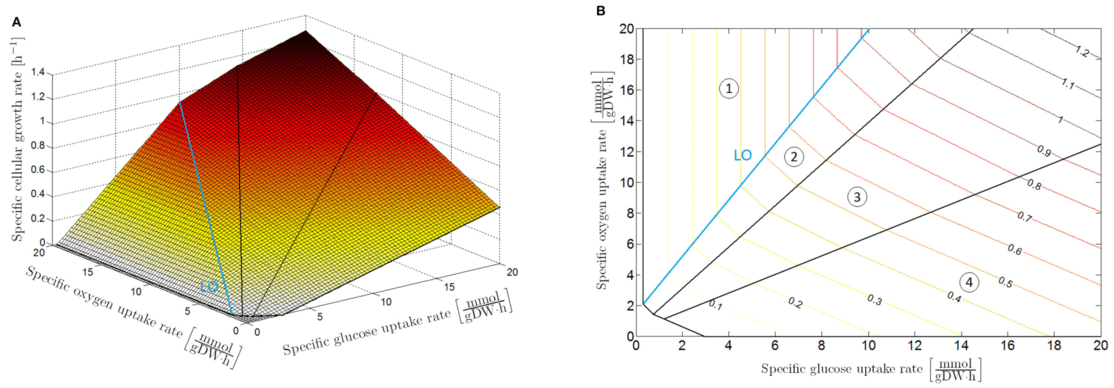
\includegraphics[width=1\columnwidth]{figures/phpp_example.png}
\caption[An example of a phenotypic phase plane for the specific growth rate as a function of oxygen and glucose uptake rates as (A) 3D plot and (B) contour plot]{An example of a phenotypic phase plane for the specific growth rate as a function of oxygen and glucose uptake rates as (A) 3D plot and (B) contour plot.}
\label{fig:phpp_example}
\end{center}
\end{figure}


\section{Flux Variability Analysis}
Flux variability analysis (FVA) finds the minimum and maximum available fluxes for each reaction while obeying the provided constraints (for example fixed glucose uptake or growth rate). FVA is mainly used  1) to evaluate the robustness of the model \cite{thiele2010functional}, 2) to find alternative optimum states \cite{mahadevan2003effects}, 3) to check flux distributions when growth is not at optimum level \cite{reed2004genome}. Many other applications of FVA can be found in the literature \cite{gudmundsson2010computationally}.

\vspace{1cm}
Flux variability analysis, similar to FBA, solves two optimization problems for each reaction:
 \begin{align}
 \ \text{max}_v / \text{min}_v \quad & v_i \\
 \ \text{subject to} \quad & S_{m \times n} \cdot v=0 \\
 \ & w^T \cdot v \geq \gamma \cdot Z_0 \\
 \ & v_{lb} \leq v \leq v_{ub}
 \end{align}
\noindent where $w$ is the objective function equals to $c$ in the problem \ref{eq:fba}, $Z_0 = w^T \cdot v_0$ describes an optimal solution to the problem \ref{eq:fba}, $\gamma$ is an indicator to check whether the FVA is done at the optimal state (where objective flux is the same and $\gamma = 1$) or any other state (where $0 \leq \gamma < 1$).

\section{Random Sampling of Solution Space}
Constraints applied to a model define a solution space, a convex polytope, where every flux distribution is accessible. Random sampling of the solution space is an unbiased tool to explore metabolic models. Mainly, Markov Chain Monte Carlo methods are used to sample this space using algorithms such as (Artificially Centered) Hit-and-Run (HRB) \cite{kiatsupaibul2011analysis, saa2016ll} algorithm, and this method has proven to be helpful in the analysis of genome-scale metabolic models \cite{schellenberger2009use}. The COBRA Toolbox \cite{heirendt2019creation} provides a workflow to generate random points by using the Hit-and-Run algorithm. Briefly, the random sampling method collects points that are uniformly distributed in the solution space and calculates the most probable flux value for each reaction.

Since the computational burden of the loopless sampling is high, generated random points in the solution space of GECKO integrated Yeast8 model include thermodynamically unfeasible states. To this sense, instead of using Hit-and-Run algorithm to sample inside the region of allowed solutions, corners of the solution space is sampled by using the workflow provided by the RAVEN Toolbox \cite{wang2018raven}.

The workflow from the RAVEN Toolbox uses the simplex method, one of the main algorithms in mathematical optimization, to calculate corners of the solution space with a random set of objective functions. Maximization of these random functions (reactions in our case) brings out the corners of the allowed solution space. This workflow also includes flux variability analysis from the COBRA Toolbox in order to prevent internal loops.

\begin{figure}[H]
\begin{center}
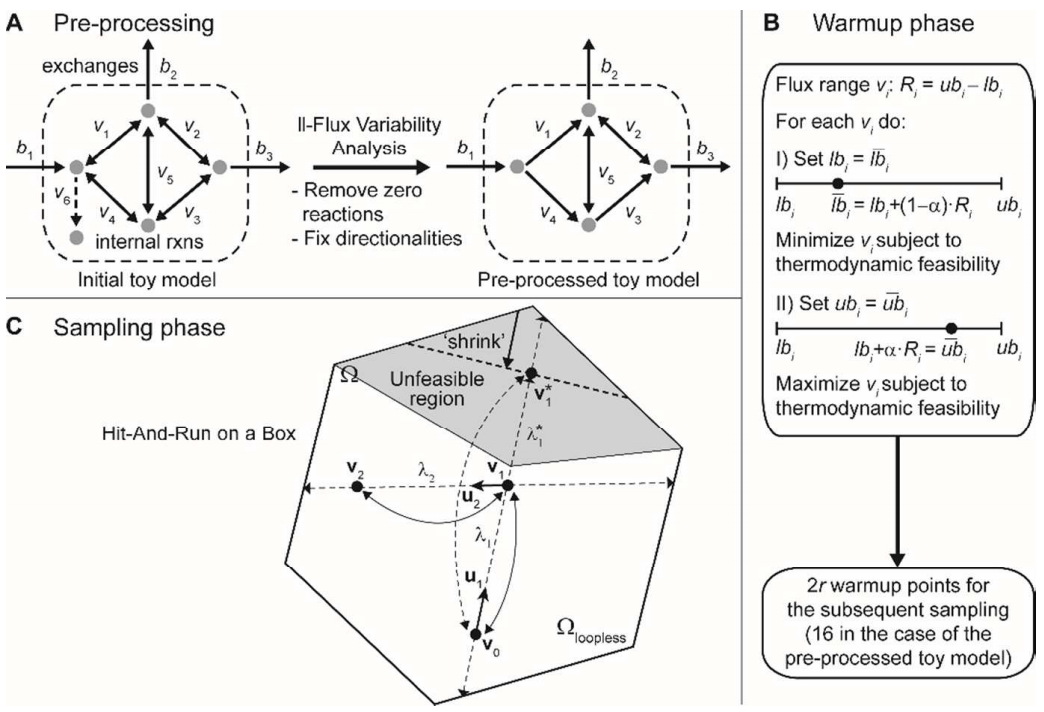
\includegraphics[width=1\columnwidth]{ll-achrb.png}
\end{center}
\caption[Workflow of the Loopless-ACHRB sampling on a toy model]{Workflow of the ll-ACHRB sampling on a toy model. A) Pre-processing phase, application of loopless-FBA to remove blocked reactions and constraining the directionalities of others. B) Warmup phase, modifying the reaction bounds to more interior space. C) Sampling phase with HRB algorithm. Figure is taken from \cite{saa2016ll}}
\label{fig:achrb}
\end{figure}


\section{Minimization of Metabolic Adjustment}
An approach for predicting mutant behavior similar to Flux Balance Analysis is based on the Minimization of Metabolic Adjustment (MOMA). The idea behind this methodology arises because a mutant is more likely to display a sub-optimal flux distribution since the selection through evolutionary adaptation has altered the genetic background of the evolved strains. Therefore the application of FBA on both wild-type and mutant strains is considered insubstantial. While the FBA method uses the objective function to present an optimal solution, MOMA choses the objective function as the minimization of the Euclidean distance between the optimal flux distribution calculated by FBA on wild type strain and the sub-optimal flux distribution of the mutant where it remains initially as close as possible to the optimal flux distribution of the wild-type.

\begin{figure}[H]
\begin{center}
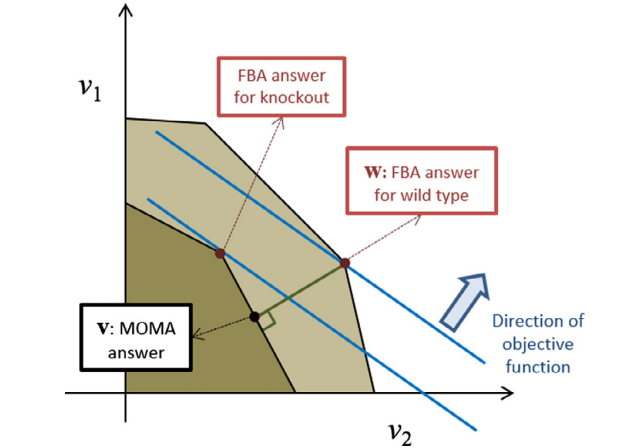
\includegraphics[width=0.8\columnwidth]{moma.png}
\caption[Comparison of FBA and MOMA flux distributions]{Comparison of FBA and MOMA flux distributions.}
\end{center}
\label{fig:moma}
\end{figure}
\noindent

Distance in the flux space is a quadratic function, thus, quadratic programming (QP) algorithm is used in MOMA instead of linear programming (LP). The COBRA Toolbox provides an approach in the form of a function called \emph{MOMA()} which can easily be implemented with command line in MATLAB. Within the function, the following FBA problem is solved first,
\begin{align}
 \ \text{max} \quad & c^T_{wt} \cdot v_{wt} \\
 \label{eq:moma_1}
 \ \text{subject to} \quad & S_{wt} \cdot v_{wt}=0 \\
 \ & lb_{wt} \leq v_{wt} \leq ub_{wt}
\end{align}
\noindent
Then the second problem is solved,
\begin{align}
 \ \text{min} \quad & \sum (v_{wt} - v_{mut})^2\\
 \label{eq:moma_2}
 \ \text{subject to} \quad & S_{wt} \cdot v_{wt}=0 \\
 \ & S_{mut} \cdot v_{mut}=0 \\
 \ & lb_{wt} \leq v_{wt} \leq ub_{wt} \\
 \ & lb_{mut} \leq v_{mut} \leq ub_{mut} \\
 \ & c^T_{wt} \cdot v_{wt} = f_{wt}
\end{align}
\noindent
where $f_{wt}$ is the optimal objective value found by FBA in the first problem.
